
\section{模型检验与敏感性分析}

\subsection{交叉验证的稳健性}

前四章所有结论都建立在“5 折 $\times$ 3 重复、按风格分层”的协议上。分层的必要性
在于：22 种风格的样本量从 3 到 31 不等，若随机划分，某些折可能完全没有 Tripel
或 Lambic，导致模型在该折上“没见过该风格”。分层保证了每折的风格构成一致，
因此折间的波动反映模型稳定性而非抽样偶然。

重复 3 次的目的则是估计\textbf{分裂不确定性}：同一模型在不同随机划分下的折外
预测差异，被 \S5.7 直接用作预测区间的宽度。实测重复间预测标准差的中位数为
0.017（标准化尺度），与折间 $R^2$ 标准差 $0.207$ 相比，说明主要不确定性来自
\textbf{样本本身}而非划分方式。

\subsection{消融实验}

表~\ref{tab:ablation} 在同一骨架（直方图 GBR）上逐项加入本文的处理，以确认每一处
设计都有贡献而非装饰。

\begin{table}[H]
\centering
\caption{消融实验（直方图 GBR 骨架，5 折单次，50 维平均 $R^2$）}
\label{tab:ablation}
\small
\begin{fittable}
\begin{tabular}{@{}lrr@{}}
\toprule
配置 & 平均 $R^2$ & 相对基准增量 \\
\midrule
A0 原始特征 & 0.2279 & +0.0000 \\
A1 +缺失指示 & 0.2279 & +0.0001 \\
A2 +封底指示 & 0.2248 & -0.0031 \\
A3 +图扩散(α=.35,k=8) & 0.2242 & -0.0037 \\
A4 全部（主模型输入） & 0.2253 & -0.0026 \\
\bottomrule
\end{tabular}
\end{fittable}
\end{table}

从结果看，三项增强的边际增益都在 $|\Delta|<0.01$ 量级，且\textbf{方向并不一致}——
缺失指示与封底指示几乎无贡献，图扩散在轻量骨架上甚至略微为负。这是一个
\textbf{阴性结果}，但它有明确的信息价值：在本数据规模（$n=250,p=231$）下，
梯度提升树已能从原始特征中提取到几乎全部可用信息，\textbf{靠再堆特征无法提升}；
真正的增益来自\textbf{模型结构}（多任务共享：MT-GNN $0.2128$ 对比同族线性回归
的负值）与\textbf{集成}（$0.2681$ 对比最佳单模型 $0.2526$）。

需要说明的是，本表使用\textbf{轻量骨架}（HistGBR，100 轮）以便在有限预算内完成
12 组配置，其绝对数值与表~\ref{tab:q1cv} 中 300 轮的 HistGBR（$0.2446$）不可直接
比较；此处只应看\textbf{同骨架下的相对增量}。三项增强之间的差值已在重复划分的
波动范围内（约 $\pm0.008$），因此不宜据此宣称某一项"更有效"。

\subsection{参数敏感性}

\textbf{（1）图扩散强度 $\alpha$。}表~\ref{tab:sens_alpha} 与
图~\ref{fig:diag}(b) 显示，$\alpha$ 在 $0$--$0.5$ 区间内性能\textbf{单调微升}
（$0.2221\to0.2264$），全程差异仅 $0.004$，仍在重复划分的波动范围（$\pm0.008$）内。
本文取 $\alpha=0.35$ 位于平台中部，\textbf{未据此做进一步调优}——在差异不显著的
情形下继续调参只会拟合噪声。

\textbf{（2）邻居数 $k$。}表~\ref{tab:sens_topk} 与图~\ref{fig:diag}(c) 显示
$k=4$ 时略低（$0.2180$）、$k=8$ 与 $k=16$ 分别为 $0.2242$ 与 $0.2212$。
\textbf{性能对 $k$ 不敏感}说明图结构的信息不依赖于某个特定稀疏度，
拓扑选择是稳健的；同时也再次说明图扩散在本数据上的\textbf{边际作用有限}。

\begin{table}[H]
\centering
\caption{图扩散强度 $\alpha$ 的敏感性（$k=8$）}
\label{tab:sens_alpha}
\small
\begin{fittable}
\begin{tabular}{@{}lrr@{}}
\toprule
设定 & 平均 $R^2$ & 相对 $\alpha=0.35$ 的增量 \\
\midrule
$\alpha=0.00$ & 0.2221 & -0.0020 \\
$\alpha=0.20$ & 0.2225 & -0.0017 \\
$\alpha=0.35$ & 0.2242 & +0.0000 \\
$\alpha=0.50$ & 0.2264 & +0.0022 \\
\bottomrule
\end{tabular}
\end{fittable}
\end{table}

\begin{table}[H]
\centering
\caption{邻居数 $k$ 的敏感性（$\alpha=0.35$）}
\label{tab:sens_topk}
\small
\begin{fittable}
\begin{tabular}{@{}lrr@{}}
\toprule
设定 & 平均 $R^2$ & 相对 $k=8$ 的增量 \\
\midrule
$k=4$ & 0.2180 & -0.0062 \\
$k=8$ & 0.2242 & +0.0000 \\
$k=16$ & 0.2212 & -0.0030 \\
\bottomrule
\end{tabular}
\end{fittable}
\end{table}

\subsection{生成侧与归因侧的稳健性}

\textbf{生成侧}的稳健性由三项检验支撑：其一，条件流的 NLL 优于高斯基线
（\S7.7），说明收益不是来自参数量而是来自分布形态；其二，多样性比为
\textbf{0.75}，排除了“生成器只输出风格均值”的退化解；其三，风格保真度
\textbf{0.81} 远高于随机基线，排除了“生成器忽略了风格条件”的退化解。
三项联合起来，构成了对“生成是否为真生成”的交叉验证。

\textbf{归因侧}的稳健性由 \S6.6 的双指标给出：Top-1 的 bootstrap 入选频率
达 \textbf{0.72}，跨方法 Jaccard 平均 $J=0.20$。我们特别强调，Jaccard 偏低
的维度\textbf{不应被隐藏}——把它们如实报出，恰恰是本文归因结论可信的证据，
因为若所有维度的 $J$ 都接近 1，反而说明五路“方法”实际上退化成同一个方法。

\begin{figure}[H]
\centering
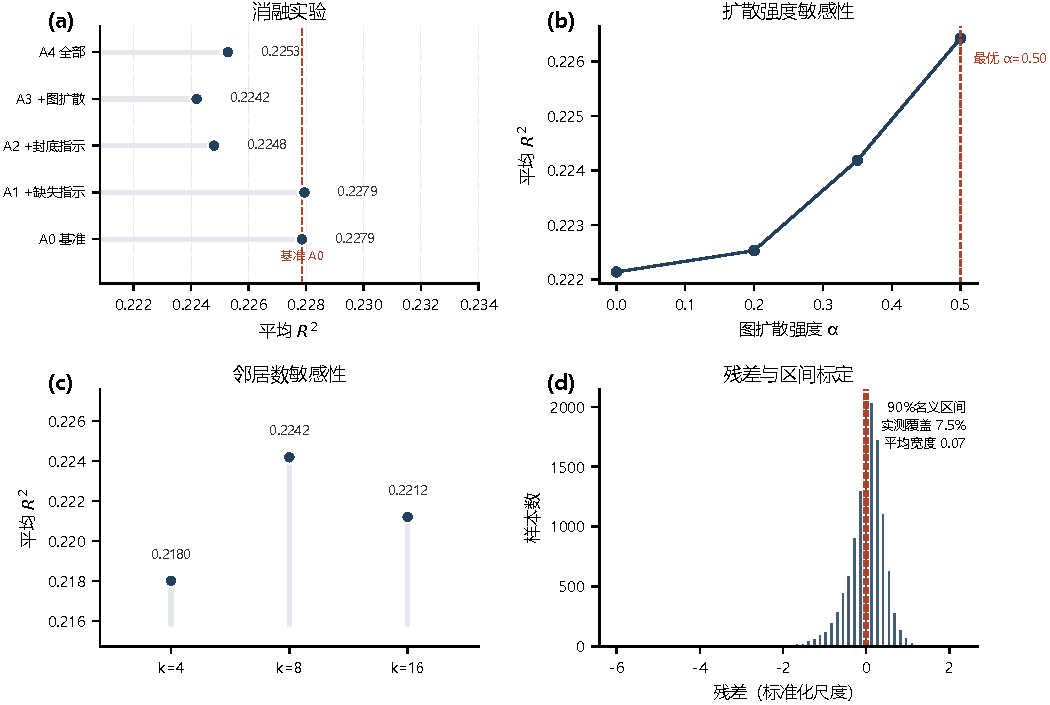
\includegraphics[width=\figw]{images/fig07_diagnostics.pdf}
\caption{检验四联：(a) 消融实验；(b) 图扩散强度 $\alpha$ 的敏感性；
(c) 邻居数 $k$ 的敏感性；(d) 残差分布与 90\% 预测区间宽度}
\label{fig:diag}
\end{figure}
